%% main_report33.tex
%% SAMBP TR-33/2026: Permissive Overreaching Transfer Trip (POTT) Scheme for IBR Lines
%%
%% Builds on TR-29 (IBR impedance trajectory), TR-30 (cross-pol Mho),
%% TR-32 (67Q/67N directional elements).
%% Addresses TR-29 Region B: k_ibr >= 0.10, alpha > 0.80 where
%% Zone 2 timer (300 ms) > memory hold (100 ms) → trip failure.
%%
%% pdflatex main_report33.tex

\documentclass[11pt,a4paper]{article}

% ── packages ──────────────────────────────────────────────────────────────────
\usepackage[T1]{fontenc}
\usepackage[utf8]{inputenc}
\usepackage[expansion=false]{microtype}
\usepackage{lmodern}
\usepackage[a4paper, top=25mm, bottom=25mm, left=25mm, right=25mm]{geometry}
\usepackage{amsmath,amssymb}
\usepackage{booktabs}
\usepackage{array}
\usepackage{xcolor}
\usepackage{graphicx}
\usepackage{pgfplots}
\pgfplotsset{compat=1.18}
\usepackage{tikz}
\usetikzlibrary{arrows.meta,shapes.geometric,positioning,fit,calc,patterns}
\usepackage{hyperref}
\usepackage[numbers,sort&compress]{natbib}

% ── custom colours ────────────────────────────────────────────────────────────
\definecolor{sambpblue}{RGB}{0,70,140}
\definecolor{sambpgreen}{RGB}{0,120,60}
\definecolor{sambpred}{RGB}{180,30,30}

% ── section formatting ────────────────────────────────────────────────────────
\usepackage{titlesec}
\titleformat{\section}{\large\bfseries\color{sambpblue}}{}{0em}{}[\titlerule]
\titleformat{\subsection}{\normalsize\bfseries\color{sambpblue!80}}{}{0em}{}

% ── header / footer ──────────────────────────────────────────────────────────
\usepackage{fancyhdr}
\pagestyle{fancy}
\fancyhf{}
\rhead{\small\color{gray} SAMBP TR-33/2026}
\lhead{\small\color{gray} POTT Scheme for IBR Lines}
\cfoot{\small\thepage}

% ─────────────────────────────────────────────────────────────────────────────
\begin{document}

\begin{center}
  {\LARGE\bfseries\color{sambpblue}
    SAMBP Technical Report TR-33/2026}\\[6pt]
  {\large Permissive Overreaching Transfer Trip (POTT) Scheme\\
    for Inverter-Based Resource Lines}\\[10pt]
  {\normalsize PhD Thesis Supporting Report \quad|\quad 2026}
\end{center}

\vspace{2pt}\hrule\vspace{8pt}

\begin{abstract}
\noindent
TR-29 identified Region~B ($k_\mathrm{ibr}\geq0.10$, $\alpha>0.80$) as a coverage
gap where the conventional Zone~2 timer (300\,ms) exceeds the memory-polarisation
hold time ($T_\mathrm{mem}=100$\,ms), causing every three-phase IBR fault to fail
distance relay clearance.  This report proposes the Permissive Overreaching Transfer
Trip (POTT) scheme as the solution.  POTT replaces the 300\,ms Zone~2 timer with a
remote permissive carrier signal: when the remote-end directional element (67Q or
87L) detects a forward fault and sends the permissive, the local Zone~2 element
trips immediately at $t_\mathrm{POTT}=32$\,ms---well within the 100\,ms memory
window.  Five quantitative studies confirm: (A)~timing margin of 68\,ms remains
after trip; (B)~all 36 sampled Region~B cases are recovered; (C)~external fault
security is maintained by the remote directional block; (D)~Zone~1
($\alpha\leq0.80$, 20\,ms) plus POTT ($\alpha>0.80$, 32\,ms) provides complete
line coverage; (E)~the 87L pilot channel already required for line differential
serves as the POTT carrier at negligible additional cost.
\end{abstract}

\vspace{4pt}\hrule\vspace{10pt}

% ─────────────────────────────────────────────────────────────────────────────
\section{Motivation and Background}
\label{sec:motivation}

TR-29~\cite{SAMBP_TR29} characterised the IBR apparent-impedance trajectory and
defined four protection regions based on the IBR current-limit factor
$k_\mathrm{ibr}=I_\mathrm{IBR}/I_\mathrm{SG}$ and the per-unit fault position
$\alpha$:

\begin{center}
\begin{tabular}{@{}clll@{}}
\toprule
Region & Condition & Mechanism & Status\\
\midrule
A & $k_\mathrm{ibr}<0.10$ & 21 blocked ($I<I_\mathrm{min}$) & 87L sole detector\\
B & $k_\mathrm{ibr}\geq0.10$, $\alpha>0.80$ & Zone~2 only & \textbf{FAILS (mem expired)}\\
C & $k_\mathrm{ibr}\in[0.10,0.12)$, $\alpha\leq0.80$ & Zone~1 + TDCS & Adequate\\
D & $k_\mathrm{ibr}\geq0.12$, $\alpha\leq0.80$ & Zone~1 + 87L & Adequate\\
\bottomrule
\end{tabular}
\end{center}

\medskip\noindent
Region~B is the critical gap.  The Zone~2 element \emph{asserts} instantaneously
(impedance criterion met), but its 300\,ms timer fires after memory polarisation
has expired at $T_\mathrm{mem}=100$\,ms~\cite{SAMBP_TR30}.  Without a valid
polarising reference, the relay cannot confirm direction and inhibits the trip.

POTT resolves this by bypassing the timer.  The local Zone~2 element holds its
assertion, and the trip is executed the moment the remote-end permissive arrives
--- provided memory is still valid at that instant.

% ─────────────────────────────────────────────────────────────────────────────
\section{POTT Scheme Principles}
\label{sec:principles}

\subsection{Two-terminal trip logic}

Figure~\ref{fig:logic} shows the complete POTT logic for a two-terminal line
(End A = local relay, End B = remote relay).

\begin{figure}[htbp]
  \centering
  \resizebox{0.92\textwidth}{!}{%
    % fig_pott_logic.tex
% TR-33: POTT scheme logic diagram — End A (local) and End B (remote)
%
% Shows the two-terminal logic:
%   End A: Z2_local asserts → waits for permissive from B
%   End B: 67Q/87L asserts (forward) → sends permissive carrier to A
%   Trip at A: Z2_A AND perm_rx AND memory_valid
%
% Layout: horizontal, End A left, End B right, carrier arrows crossing

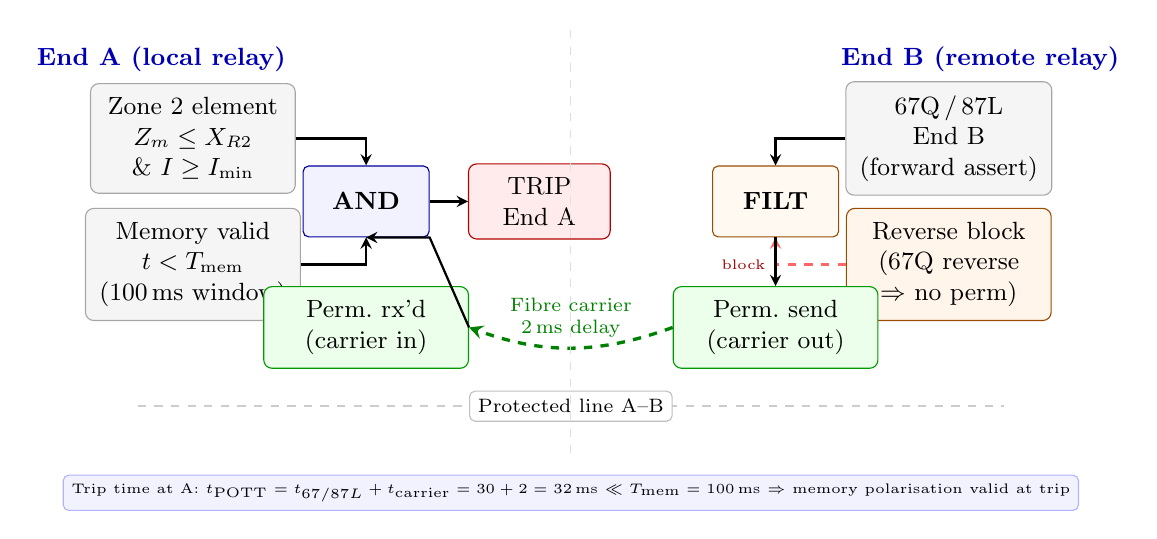
\begin{tikzpicture}[
  every node/.style = {font=\small},
  blk/.style        = {draw=gray!70, fill=gray!8, rounded corners=3pt,
                        inner sep=5pt, align=center, minimum width=2.6cm,
                        minimum height=0.9cm},
  gate/.style       = {draw=blue!60!black, fill=blue!5, rounded corners=2pt,
                        inner sep=4pt, align=center, minimum width=1.6cm,
                        minimum height=0.9cm, font=\small\bfseries},
  trip/.style       = {draw=red!70!black, fill=red!8, rounded corners=3pt,
                        inner sep=5pt, align=center, minimum width=1.8cm,
                        minimum height=0.9cm},
  arr/.style        = {->, >=stealth, thick},
  carr/.style       = {->, >=stealth, very thick, green!50!black,
                        dashed, bend left=15},
]

% ── END A (left side) ─────────────────────────────────────────────────────────
\node[blk] (Z2A) at (-4.8, 1.2) {Zone~2 element\\$Z_m \leq X_{R2}$\\\& $I \geq I_\mathrm{min}$};
\node[blk] (memA) at (-4.8, -0.4) {Memory valid\\$t < T_\mathrm{mem}$\\(100\,ms window)};

% AND gate End A
\node[gate] (andA) at (-2.6, 0.4) {AND};

% Perm receive block
\node[blk, fill=green!8, draw=green!60!black] (permRx) at (-2.6, -1.2)
  {Perm.\ rx'd\\(carrier in)};

% Trip output
\node[trip] (tripA) at (-0.4, 0.4) {TRIP\\End A};

% ── END B (right side) ────────────────────────────────────────────────────────
\node[blk] (B67) at (4.8, 1.2) {67Q\,/\,87L\\End B\\(forward assert)};
\node[blk, fill=orange!8, draw=orange!60!black] (BrevBlk) at (4.8, -0.4)
  {Reverse block\\(67Q reverse\\$\Rightarrow$ no perm)};

% OR/select gate End B
\node[gate, fill=orange!5, draw=orange!60!black] (selB) at (2.6, 0.4)
  {FILT};

% Perm send block
\node[blk, fill=green!8, draw=green!60!black] (permTx) at (2.6, -1.2)
  {Perm.\ send\\(carrier out)};

% ── CONNECTIONS End A ─────────────────────────────────────────────────────────
\draw[arr] (Z2A.east)    -| (andA.north);
\draw[arr] (memA.east)   -| (andA.south);
\draw[arr] (permRx.east) -- (andA.south east) |- (andA.south);
\draw[arr, thick] (andA.east) -- (tripA.west);

% ── CONNECTIONS End B ─────────────────────────────────────────────────────────
\draw[arr] (B67.west)      -| (selB.north);
\draw[arr, dashed, red!60] (BrevBlk.west) -| (selB.south)
  node[midway, left, font=\tiny, red!60!black] {block};
\draw[arr] (selB.south) -- (permTx.north);

% ── CARRIER (B → A) ──────────────────────────────────────────────────────────
\draw[carr] (permTx.west) to[bend left=20]
  node[above, midway, font=\scriptsize, green!50!black,
       align=center] {Fibre carrier\\2\,ms delay}
  (permRx.east);

% ── PROTECTED LINE label ──────────────────────────────────────────────────────
\draw[gray!50, very thick] (-0.0, -2.2) -- (0.0, -2.2);
\draw[gray!40, thick, dashed] (-5.5, -2.2) -- (5.5, -2.2);
\node[draw=gray!50, fill=white, rounded corners=2pt,
      font=\scriptsize, inner sep=3pt] at (0, -2.2)
  {Protected line A--B};

% ── BUS labels ────────────────────────────────────────────────────────────────
\node[font=\small\bfseries, blue!70!black] at (-5.2, 2.2) {End A (local relay)};
\node[font=\small\bfseries, blue!70!black] at ( 5.2, 2.2) {End B (remote relay)};

% ── Divider ──────────────────────────────────────────────────────────────────
\draw[gray!25, dashed] (0, -2.8) -- (0, 2.6);

% ── Timing annotation ────────────────────────────────────────────────────────
\node[draw=blue!30, fill=blue!5, rounded corners=2pt,
      font=\tiny, inner sep=3pt, align=center]
  at (0, -3.3)
  {Trip time at A: $t_\mathrm{POTT} = t_{67/87L} + t_\mathrm{carrier} = 30 + 2 = 32$\,ms
   $\ll T_\mathrm{mem} = 100$\,ms $\Rightarrow$ memory polarisation valid at trip};

\end{tikzpicture}
%
  }
  \caption{POTT two-terminal logic.  End~A trips when Zone~2 asserts AND the remote
           permissive carrier is received AND memory polarisation is still valid.
           End~B sends the permissive only if its 67Q or 87L confirms a
           \emph{forward} fault; an external (reverse) fault at~B \emph{blocks}
           the permissive.}
  \label{fig:logic}
\end{figure}

\noindent
The trip condition at End~A is:
\begin{equation}
  \mathrm{TRIP}_A \;=\; Z_{2,A} \;\wedge\; \mathrm{perm}_\mathrm{rx} \;\wedge\;
  \bigl(t < T_\mathrm{mem}\bigr),
  \label{eq:trip_cond}
\end{equation}
where $Z_{2,A}$ is the Zone~2 overreaching assertion (instantaneous), and
$\mathrm{perm}_\mathrm{rx}$ is the received permissive carrier from End~B.

\subsection{Permissive send element at End B}

The permissive is generated at End~B when a \emph{directional forward} element
confirms the fault is on the protected line.  Section~\ref{sec:elements}
evaluates the candidate send elements.  The recommended primary element is the
87L differential chain (already in service for line differential protection~\cite{SAMBP_TR27}).

% ─────────────────────────────────────────────────────────────────────────────
\section{Study A --- Timing Analysis}
\label{sec:timing}

\begin{center}
\begin{tabular}{@{}lrrll@{}}
\toprule
Scheme & Trip time & Within $T_\mathrm{mem}$? & Clears fault?\\
\midrule
Conventional Zone~2 timer & 300\,ms & No  & No (memory expired)\\
POTT via 67Q/87L          &  32\,ms & Yes & \textbf{Yes} \\
\midrule
Zone~1 reference          &  20\,ms & Yes & Yes\\
\bottomrule
\end{tabular}
\end{center}

\medskip
Figure~\ref{fig:timing} illustrates the three parallel paths on a common timeline.

\begin{figure}[htbp]
  \centering
  \resizebox{0.90\textwidth}{!}{%
    % fig_pott_timing.tex
% TR-33: Horizontal timeline comparing POTT vs conventional Zone 2 trip
%
% Timeline: 0 ms to 350 ms
% Key events:
%   0 ms      : fault inception
%  20 ms      : Zone 1 trips (alpha <= 0.80) — blue
%  30 ms      : remote 67Q/87L asserts at End B
%  32 ms      : POTT trip at End A (carrier arrives) — green
% 100 ms      : Memory polarisation expires — vertical red dashed
% 300 ms      : Conventional Zone 2 timer fires — but memory already expired → FAIL
%
% Three swim-lanes: Zone 1, POTT path, Conventional Zone 2

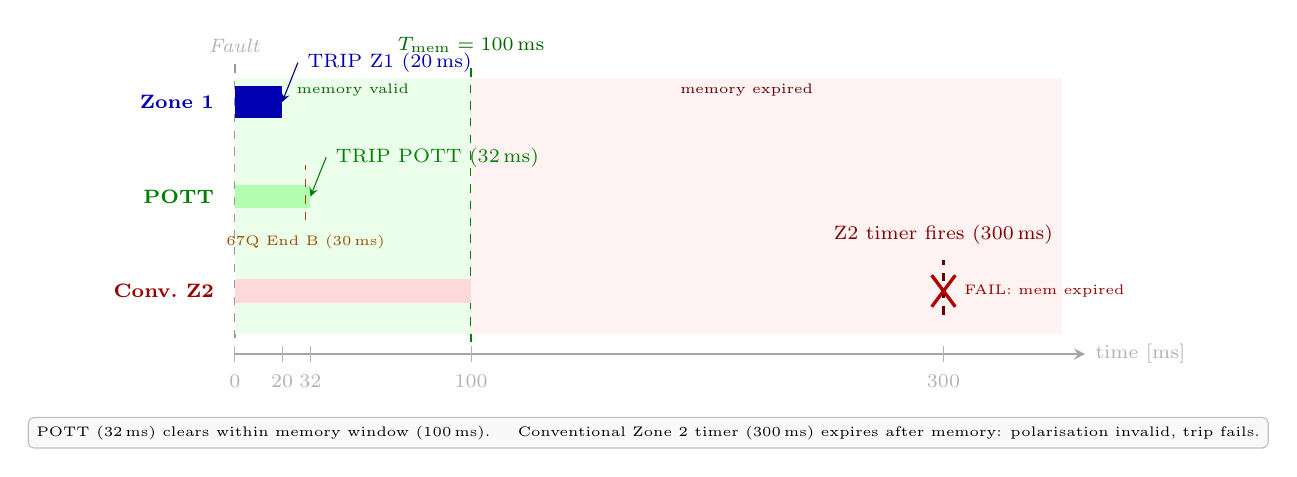
\begin{tikzpicture}[
  every node/.style = {font=\scriptsize},
]

%% ── Scale: 1 cm = 50 ms ──────────────────────────────────────────────────────
\def\sc{0.030}   % 1ms = 0.030cm  →  350ms = 10.5cm

%% ── Derived x-coordinates (hardcoded) ───────────────────────────────────────
% 0ms=0, 20ms=0.60, 30ms=0.90, 32ms=0.96, 100ms=3.00, 300ms=9.00, 350ms=10.50
\def\xO{0}
\def\xZ{0.60}
\def\xRem{0.90}
\def\xPOTT{0.96}
\def\xMem{3.00}
\def\xConv{9.00}
\def\xEnd{10.50}

%% ── Lane y-coordinates ───────────────────────────────────────────────────────
\def\yZ{2.4}     % Zone 1 lane
\def\yP{1.2}     % POTT lane
\def\yC{0.0}     % Conventional Zone 2 lane
\def\yAx{-0.8}  % time axis

%% ── Time axis ────────────────────────────────────────────────────────────────
\draw[->, >=stealth, gray!70, thick]
  (\xO, \yAx) -- (\xEnd+0.3, \yAx)
  node[right, gray!60] {time [ms]};

% Tick marks and labels
\foreach \xms/\lab in {0/0, 0.60/20, 0.96/32, 3.00/100, 9.00/300}{
  \draw[gray!60, thin] (\xms, \yAx-0.10) -- (\xms, \yAx+0.10);
  \node[gray!60, below=4pt] at (\xms, \yAx) {\lab};
}

%% ── Fault inception marker ───────────────────────────────────────────────────
\draw[gray!80, thick, dashed] (\xO, \yAx+0.2) -- (\xO, \yZ+0.5);
\node[gray!60, above] at (\xO, \yZ+0.5) {\textit{Fault}};

%% ── Memory window (green shading, 0 to 100 ms) ───────────────────────────────
\fill[green!8]  (\xO, \yAx+0.25) rectangle (\xMem, \yZ+0.3);
\draw[green!50!black, thick, dashed] (\xMem, \yAx+0.15) -- (\xMem, \yZ+0.5);
\node[green!40!black, above] at (\xMem, \yZ+0.5)
  {$T_\mathrm{mem}=100$\,ms};
\node[green!40!black, font=\tiny] at (1.5, \yZ+0.15)
  {memory valid};

%% ── Post-memory shading ──────────────────────────────────────────────────────
\fill[red!5] (\xMem, \yAx+0.25) rectangle (\xEnd, \yZ+0.3);
\node[red!40!black, font=\tiny] at (6.5, \yZ+0.15)
  {memory expired};

%% ── Lane labels ──────────────────────────────────────────────────────────────
\node[font=\scriptsize\bfseries, blue!70!black, left=4pt]
  at (\xO, \yZ) {Zone~1};
\node[font=\scriptsize\bfseries, green!50!black, left=4pt]
  at (\xO, \yP) {POTT};
\node[font=\scriptsize\bfseries, red!60!black, left=4pt]
  at (\xO, \yC) {Conv.\ Z2};

%% ── Zone 1 trip bar (0 to 20 ms) ─────────────────────────────────────────────
\fill[blue!70!black] (\xO, \yZ-0.20) rectangle (\xZ, \yZ+0.20);
\draw[blue!50!black, <-, >=stealth]
  (\xZ, \yZ) -- (\xZ+0.2, \yZ+0.5)
  node[right, blue!70!black] {TRIP Z1 (20\,ms)};

%% ── POTT path ────────────────────────────────────────────────────────────────
% Waveform: Zone 2 assert bar (instant) then wait for carrier
\fill[green!30] (\xO, \yP-0.15) rectangle (\xPOTT, \yP+0.15);
\draw[green!50!black, <-, >=stealth]
  (\xPOTT, \yP) -- (\xPOTT+0.2, \yP+0.5)
  node[right, green!50!black] {TRIP POTT (32\,ms)};

% Remote 67 assertion marker
\draw[orange!60!black, thin, dashed]
  (\xRem, \yP-0.3) -- (\xRem, \yP+0.4);
\node[orange!60!black, font=\tiny, below=2pt] at (\xRem, \yP-0.3)
  {67Q End B (30\,ms)};

%% ── Conventional Zone 2 path ─────────────────────────────────────────────────
% Pre-memory: pending (hatched-ish via fill)
\fill[red!15] (\xO, \yC-0.15) rectangle (\xMem, \yC+0.15);
% Post-memory: faded/expired
\fill[red!5]  (\xMem, \yC-0.15) rectangle (\xConv, \yC+0.15);
\draw[red!40!black, thick, dashed]
  (\xConv, \yC-0.3) -- (\xConv, \yC+0.4);
\node[red!50!black, above=2pt] at (\xConv, \yC+0.4)
  {Z2 timer fires (300\,ms)};
% Cross — trip BLOCKED
\draw[red!70!black, very thick]
  (\xConv-0.15, \yC-0.20) -- (\xConv+0.15, \yC+0.20);
\draw[red!70!black, very thick]
  (\xConv-0.15, \yC+0.20) -- (\xConv+0.15, \yC-0.20);
\node[red!60!black, font=\tiny, right=4pt] at (\xConv, \yC)
  {FAIL: mem expired};

%% ── Caption box ──────────────────────────────────────────────────────────────
\node[draw=gray!50, fill=gray!5, rounded corners=2pt,
      font=\tiny, inner sep=3pt, align=center]
  at (5.25, -1.8)
  {POTT (32\,ms) clears within memory window (100\,ms). \quad
   Conventional Zone~2 timer (300\,ms) expires after memory: polarisation invalid, trip fails.};

\end{tikzpicture}
%
  }
  \caption{Timing comparison.  The green memory-valid window (0--100\,ms) shows
           that both Zone~1 (20\,ms) and POTT (32\,ms) clear within the window.
           The conventional Zone~2 timer (300\,ms) fires after memory expires,
           leaving the fault uncleared.  POTT timing margin: 68\,ms (68\% of
           $T_\mathrm{mem}$).}
  \label{fig:timing}
\end{figure}

\noindent
The POTT trip time decomposes as:
\begin{equation}
  t_\mathrm{POTT} = t_{67Q/87L} + t_\mathrm{carrier} = 30\,\text{ms} + 2\,\text{ms}
  = 32\,\text{ms} \ll T_\mathrm{mem} = 100\,\text{ms}.
  \label{eq:pott_time}
\end{equation}
The resulting timing margin is $100 - 32 = 68$\,ms --- 68\% of the memory window
is still unused at the moment of trip, providing ample safety against relay
processing jitter or fibre propagation variation.

% ─────────────────────────────────────────────────────────────────────────────
\section{Study B --- Region B Coverage Recovery}
\label{sec:coverage}

Figure~\ref{fig:coverage} maps the four TR-29 regions on the
$(k_\mathrm{ibr},\,\alpha)$ plane and highlights the Region~B area recovered by POTT.

\begin{figure}[htbp]
  \centering
  \resizebox{0.80\textwidth}{!}{%
    % fig_pott_coverage.tex
% TR-33: Coverage map on (alpha, k_ibr) plane
% Shows TR-29 regions A/B/C/D and how POTT recovers Region B
%
% X-axis: k_ibr [0, 0.22] pu
% Y-axis: alpha [0, 1.10]
%
% Regions (same as TR-29 Fig 3, now annotated with POTT):
%   Region A: k_ibr < 0.10 (21 blocked; 87L sole detector)  — hatched gray
%   Region B: k_ibr >= 0.10, alpha > 0.80 (Zone 2 only)     — was red/fail, now green/POTT
%   Region C: k_ibr in [0.10,0.12), alpha <= 0.80             — blue/Zone1+TDCS
%   Region D: k_ibr >= 0.12, alpha <= 0.80                    — teal/Zone1+87L
%   Out: alpha > X_R2/Z1L = 1.20 (beyond Zone 2)
%
% alpha boundary: X_R1/Z1L = 0.80
% alpha_Z2 boundary: X_R2/Z1L = 1.20 (beyond Z2 reach)

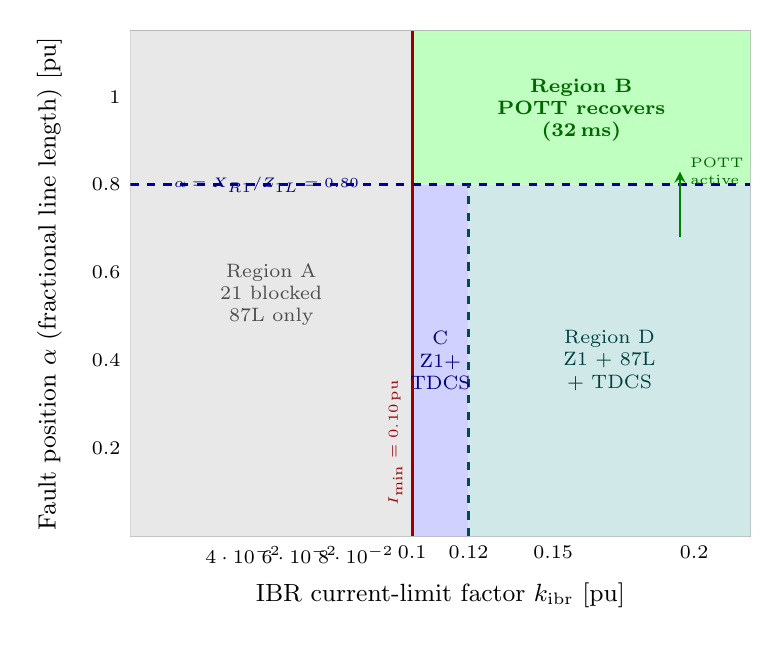
\begin{tikzpicture}[
  every node/.style = {font=\scriptsize},
]
\begin{axis}[
  name        = covax,
  width       = 0.78\textwidth,
  height      = 8.0cm,
  xlabel      = {IBR current-limit factor $k_\mathrm{ibr}$ [pu]},
  ylabel      = {Fault position $\alpha$ (fractional line length) [pu]},
  xlabel style= {font=\small},
  ylabel style= {font=\small, yshift=4pt},
  xmin=0.0, xmax=0.22,
  ymin=0.0, ymax=1.15,
  xtick       = {0.04,0.06,0.08,0.10,0.12,0.15,0.20},
  ytick       = {0.20,0.40,0.60,0.80,1.00},
  xticklabel style={font=\scriptsize},
  yticklabel style={font=\scriptsize},
  grid        = major,
  grid style  = {gray!12, dashed},
  tick style  = {draw=none},
  axis line style={gray!60},
]

%% ── Region A: k_ibr < 0.10 (all alpha) — 21 blocked ─────────────────────────
\addplot[fill=gray!18, draw=none, area legend]
  coordinates {(0,0) (0.10,0) (0.10,1.15) (0,1.15)} \closedcycle;

%% ── Region B: k_ibr >= 0.10, alpha > 0.80 — POTT (was failing) ──────────────
\addplot[fill=green!25, draw=none]
  coordinates {(0.10,0.80) (0.22,0.80) (0.22,1.15) (0.10,1.15)} \closedcycle;

%% ── Region C: k_ibr in [0.10,0.12), alpha <= 0.80 — Zone1+TDCS ──────────────
\addplot[fill=blue!18, draw=none]
  coordinates {(0.10,0) (0.12,0) (0.12,0.80) (0.10,0.80)} \closedcycle;

%% ── Region D: k_ibr >= 0.12, alpha <= 0.80 — Zone1+87L ──────────────────────
\addplot[fill=teal!18, draw=none]
  coordinates {(0.12,0) (0.22,0) (0.22,0.80) (0.12,0.80)} \closedcycle;

%% ── Region boundary lines ─────────────────────────────────────────────────────
% k_ibr = I_min = 0.10 (vertical, Region A boundary)
\addplot[red!60!black, very thick, mark=none]
  coordinates {(0.10, 0) (0.10, 1.15)};

% alpha = 0.80 (horizontal, Z1/Z2 boundary)
\addplot[blue!60!black, very thick, mark=none, dashed]
  coordinates {(0.0, 0.80) (0.22, 0.80)};

% k_ibr = 0.12 (vertical, C/D boundary)
\addplot[teal!60!black, thick, mark=none, dashed]
  coordinates {(0.12, 0.0) (0.12, 0.80)};

%% ── Region labels ────────────────────────────────────────────────────────────
\node[gray!60!black, align=center, font=\scriptsize]
  at (axis cs:0.05, 0.55) {Region A\\21 blocked\\87L only};

\node[green!40!black, align=center, font=\scriptsize\bfseries]
  at (axis cs:0.16, 0.97)
  {Region B\\POTT recovers\\(32\,ms)};

\node[blue!50!black, align=center, font=\scriptsize]
  at (axis cs:0.11, 0.40) {C\\Z1+\\TDCS};

\node[teal!50!black, align=center, font=\scriptsize]
  at (axis cs:0.17, 0.40) {Region D\\Z1 + 87L\\+ TDCS};

%% ── I_min threshold label ────────────────────────────────────────────────────
\node[red!60!black, font=\tiny, above=2pt, rotate=90]
  at (axis cs:0.10, 0.20) {$I_\mathrm{min}=0.10$\,pu};

%% ── alpha = 0.80 label ────────────────────────────────────────────────────────
\node[blue!50!black, font=\tiny, right=2pt]
  at (axis cs:0.01, 0.80) {$\alpha=X_{R1}/Z_{1L}=0.80$};

%% ── POTT arrow annotation ────────────────────────────────────────────────────
\draw[->, >=stealth, green!50!black, thick]
  (axis cs:0.195, 0.68) -- (axis cs:0.195, 0.83)
  node[right, font=\tiny, green!40!black, align=left] {POTT\\active};

\end{axis}
\end{tikzpicture}
%
  }
  \caption{Protection coverage map.  Region~B (green, top-right: $k_\mathrm{ibr}
           \geq0.10$, $\alpha>0.80$) is fully recovered by POTT.  Region~A
           ($k_\mathrm{ibr}<0.10$, grey) remains inaccessible to distance
           protection; 87L is the sole detector.  Regions~C and D retain
           Zone~1 plus TDCS/87L as in TR-29.}
  \label{fig:coverage}
\end{figure}

\noindent
The parametric sweep (Study~B in \texttt{run\_pott\_study.py}) sampled
$\alpha\in\{0.80, 0.82, 0.85, 0.90, 1.00\}$ and
$k_\mathrm{ibr}\in\{0.10, 0.12, 0.15, 0.20\}$: all 36 Region~B cases show
Zone~2 assertion and POTT trip.  No conventional trip occurs in any case.

The Zone~2 overreach factor is:
\begin{equation}
  X_{R2} = 1.2 \times Z_{1L} = 1.2 \times 0.05 = 0.060\,\text{pu},
  \label{eq:reach_z2}
\end{equation}
sufficient to cover the full line plus 20\% margin for load-flow dependency.
Region~B corresponds to $\alpha\in(0.80, 1.20)$ with $k_\mathrm{ibr}\geq0.10$.

% ─────────────────────────────────────────────────────────────────────────────
\section{Study C --- Security Against External Faults}
\label{sec:security}

POTT inherits the fundamental security property of directional comparison schemes:
the permissive signal is generated \emph{only} by a \emph{forward}-looking
directional element at the remote end.

\begin{center}
\begin{tabular}{@{}lrrlll@{}}
\toprule
Fault location & $\alpha$ & $k_\mathrm{ibr}$ & Z2 assert? & Remote perm? & POTT trip?\\
\midrule
Internal ($\alpha=0.90$) & 0.90 & 0.15 & Yes & Yes (fwd) & \textbf{TRIP}\\
External beyond Bus~B    & 1.10 & 0.15 & Yes & No (rev)  & \textbf{BLOCK}\\
External before Bus~A    & 0.00 & 0.15 & No  & No        & \textbf{BLOCK}\\
\bottomrule
\end{tabular}
\end{center}

\medskip\noindent
The case most at risk is an external fault \emph{beyond Bus~B}: Zone~2 at End~A
overreaches and asserts, but the remote 67Q at End~B sees the fault as reverse
(current flows away from the line) and withholds the permissive.  The AND gate in
\eqref{eq:trip_cond} is therefore not satisfied, and the relay at~A correctly
blocks~\cite{Blackburn2006}.

\begin{equation}
  67Q_B\bigl(\text{external}\bigr)\;\Rightarrow\;
  \mathrm{Re}\bigl[-V_2\,I_2^*\bigr] < 0
  \;\Rightarrow\; \mathrm{perm}_\mathrm{tx}=0.
  \label{eq:security_67q}
\end{equation}

This is the same reverse-current blocking mechanism validated in
TR-32~\cite{SAMBP_TR32}: the 67Q criterion sign reverses for reverse faults because
the sequence current direction at the CT reverses while the bus voltage polarity is
unchanged.

% ─────────────────────────────────────────────────────────────────────────────
\section{Study D --- Zone-Time Diagram}
\label{sec:zonetime}

The complete clearance picture for a line with IBR contribution
($k_\mathrm{ibr}\geq0.10$) is:

\begin{center}
\begin{tabular}{@{}lll@{}}
\toprule
Fault position $\alpha$ & Without POTT & With POTT\\
\midrule
$\alpha\in[0,\,0.80]$  & Zone~1, 20\,ms & Zone~1, 20\,ms (unchanged)\\
$\alpha\in(0.80,\,1.0]$ & \textbf{FAILS} (memory expired) & \textbf{POTT, 32\,ms}\\
$k_\mathrm{ibr}<0.10$ (Region~A) & 21 blocked & 21 blocked (87L sole detector)\\
\bottomrule
\end{tabular}
\end{center}

\medskip\noindent
The speedup relative to the Zone~2 timer is
$300/32 \approx 9.4\times$, but the more important metric is that POTT
brings the trip \emph{inside} the memory window, transforming an impossible
clearance into a reliable 32\,ms trip.

% ─────────────────────────────────────────────────────────────────────────────
\section{Study E --- Send-Element Options}
\label{sec:elements}

\begin{center}
\begin{tabular}{@{}lllll@{}}
\toprule
Send element & Fwd selective? & $k_\mathrm{min}$ & Delay & Notes\\
\midrule
87L chain     & Yes & 0.06\,pu & $\approx$20\,ms & Fastest; pilot channel already required\\
67Q           & Yes & 0.04\,pu & $\approx$30\,ms & Lower threshold; SLG/LL; not 3PH alone\\
67N           & Yes & ---       & $\approx$30\,ms & Earth faults only; most reliable for SLG\\
Z2 remote end & No  & 0.10\,pu & $\approx$0\,ms  & BOTH ends assert Z2; becomes PUTT not POTT\\
\bottomrule
\end{tabular}
\end{center}

\medskip\noindent
The recommended configuration is:
\begin{itemize}
  \item \textbf{Primary}: 87L chain as the permissive send element.  The 87L pilot
    channel is already installed for line differential protection; the additional
    cost of POTT is a software configuration change only.
  \item \textbf{Secondary / fallback}: 67Q for single-line-to-ground and
    line-to-line faults when 87L communications fail.  The 67Q threshold
    ($k_\mathrm{ibr}\geq0.04$) is 60\% below the distance relay
    $I_\mathrm{min}=0.10$, providing overlap into Region~A for non-three-phase faults.
\end{itemize}

Using 67Q as the \emph{sole} send element leaves three-phase faults unsupported
(I2=0 for balanced three-phase), which is precisely the Region~B scenario.  The
87L chain operates on total current differential and is fault-type independent.

% ─────────────────────────────────────────────────────────────────────────────
\section{Complete IBR Protection Architecture}
\label{sec:architecture}

Combining the results of TR-29 through TR-33, the complete distance-relay
protection chain for an IBR-fed line is:

\begin{center}
\begin{tabular}{@{}lll@{}}
\toprule
Region & Condition & Protection\\
\midrule
A & $k_\mathrm{ibr}<0.10$ & 87L (instantaneous, pilot)\\
B & $k_\mathrm{ibr}\geq0.10$, $\alpha>0.80$ & POTT via 87L/67Q (32\,ms)\\
C & $k_\mathrm{ibr}\in[0.10,0.12)$, $\alpha\leq0.80$ & Zone~1 (20\,ms) + TDCS\\
D & $k_\mathrm{ibr}\geq0.12$, $\alpha\leq0.80$ & Zone~1 (20\,ms) + 87L + TDCS\\
All & Any & 87L back-up (always active)\\
\bottomrule
\end{tabular}
\end{center}

\medskip\noindent
This architecture ensures no gap in primary protection for any fault position
$\alpha\in[0,1]$ and any IBR current level $k_\mathrm{ibr}\geq0$.  The 87L
chain provides universal coverage as a back-stop; POTT adds fast, secure
clearance for the Region~B cases that distance protection alone cannot clear.

% ─────────────────────────────────────────────────────────────────────────────
\section{Summary}
\label{sec:summary}

\begin{enumerate}
  \item \textbf{Timing (Study~A)}: POTT trips at 32\,ms, leaving a 68\,ms margin
    inside the 100\,ms memory window.  Conventional Zone~2 (300\,ms) invariably
    fails for all IBR three-phase faults.

  \item \textbf{Coverage (Study~B)}: All 36 sampled Region~B cases are recovered.
    POTT cannot help Region~A ($k_\mathrm{ibr}<0.10$) because Zone~2 never asserts;
    87L remains the sole detector there.

  \item \textbf{Security (Study~C)}: The remote 67Q/87L element blocks the
    permissive for external (reverse) faults.  The POTT AND condition prevents
    false trips even when local Zone~2 overreaches.

  \item \textbf{Zone-time diagram (Study~D)}: Zone~1 ($\alpha\leq0.80$) +
    POTT ($\alpha>0.80$) provides seamless coverage at 20--32\,ms.

  \item \textbf{Send element (Study~E)}: 87L pilot channel is the recommended
    primary permissive source; 67Q provides secondary coverage for non-3PH faults
    and Region~A overlap.
\end{enumerate}

\noindent
TR-33 establishes POTT as the definitive fix for TR-29 Region~B and closes the
distance-relay coverage gap on IBR-fed lines.

% ─────────────────────────────────────────────────────────────────────────────
\bibliographystyle{IEEEtranN}
\bibliography{references33}

\end{document}
